\documentclass[]{standalone}
\usepackage{tikz}
\usepackage{palatino}
\usetikzlibrary{shapes,arrows,trees,calc}
\usepackage{tikz}
\usetikzlibrary{trees,shapes}
\begin{document}
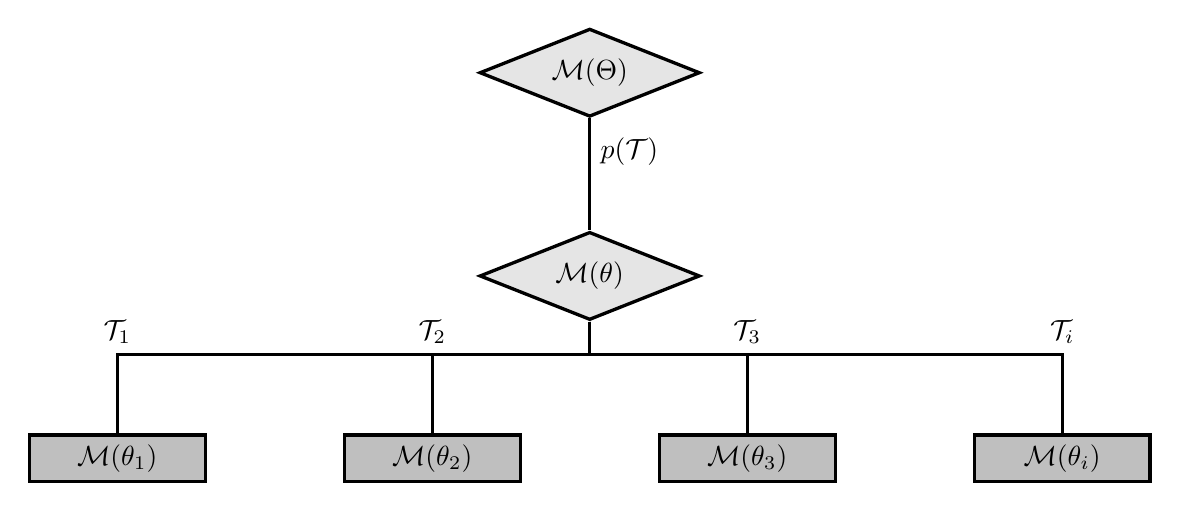
\begin{tikzpicture}[
    test/.style={
        % Node style
        diamond, 
        aspect=2.5,
        very thick,
        draw=black,
        fill=gray!20,
        text width=1.1cm,
        align=center, 
        anchor=north},
    dec/.style={
        rectangle,
        very thick,
        draw=black,
        fill=gray!50,
        text width=2cm,
        text centered, 
        anchor=north
    },
    % Children and edges style
    edge from parent/.style={
        very thick,
    draw=black},
    edge from parent fork down,
    level 1/.style={
        sibling distance=4cm,
        level distance=2cm}
    ]

%\node (t1) [test] {$\mathcal{M}(\Theta)$} 
%	child { node (t2) [dec] {$\mathcal{M}(\theta)$}  
%            edge from parent node[above] {$p(\mathcal{T})$}
%    
%	child { node (t2) [dec] {$\mathcal{M}(\theta_1)$}  
%            edge from parent node[above] {$\mathcal{T}_1$}
%    }
%    child { node (t2) [dec] {$\mathcal{M}(\theta_1)$}  
%            edge from parent node[above] {$\mathcal{T}_1$}
%    }
%    child{ node (d1) [dec] {$\mathcal{M}(\theta_2)$} edge from parent node[above] {$\mathcal{T}_2$} }
%    child{ node (d1) [dec] {$\mathcal{M}(\theta_3)$} edge from parent node[above] {$\mathcal{T}_3$} } 
%    child{ node (d1) [dec] {$\mathcal{M}(\theta_i)$} edge from parent node[above] {$\mathcal{T}_i$} }};


\node (t1) [test] {$\mathcal{M}(\Theta)$} 
    child { node (t2) [test] {$\mathcal{M}(\theta)$}  
        child { node (t3) [dec] {$\mathcal{M}(\theta_1)$} 
            edge from parent node[above] {$\mathcal{T}_1$}
        }
        child { node (d2) [dec] {$\mathcal{M}(\theta_2)$}  edge from parent node[above] {$\mathcal{T}_2$} }
        child { node (d2) [dec] {$\mathcal{M}(\theta_3)$}  edge from parent node[above] {$\mathcal{T}_3$} }
		child { node (d2) [dec] {$\mathcal{M}(\theta_i)$}  edge from parent node[above] {$\mathcal{T}_i$} }
            edge from parent node[right] {$p(\mathcal{T})$}
    }
     %
;
\end{tikzpicture}
\end{document}
